%!TEX root = thesis.tex

%%%%%%%%%%%%%%%%%%%%%%%%%%%%%%%%
% intro.tex: Introduction to the thesis
%%%%%%%%%%%%%%%%%%%%%%%%%%%%%%%%
\chapter{Introduction}
\label{chap:intro}


A galaxy's morphology is the culmination of its formation, interactions, and evolution through environmental and internal processes. It is a snapshot into the current state of a galaxy's life as well as a window to its past. The insights gleaned through the study of galaxy morphology have radically changed our view of the universe since the time of Edwin Hubble. 


Astronomers have made use of visual galaxy morphologies to understand the dynamical structure of these systems for nearly ninety years 
\citep[e.g.,][]{Hubble1936, 
			deVaucouleurs1959,
			Sandage1961, 
			vandenBergh1976, 
			NairAbraham2010, 
			Baillard2011}. 
The division between early-type and late-type (see Section \ref{chap1: standard morphologies}) systems corresponds, for example, to a wide range of parameters from mass and luminosity, to environment, color, and star formation history 
\citep[e.g.,][]{Kormendy1977,  
			Dressler1980, 
			Strateva2001, 
			Blanton2003a, 
			Kauffman2003, 
			Nakamura2003, 
			Shen2003, 
			Peng2010}; 
while detailed observations of morphological features such as bars and bulges provide information about the history of {}their host systems 
\citep[e.g.,][]{KK04, 
			Elmegreen2008, 
			Sheth2008, 
			Masters2010, 
			Simmons2014}. 
Modern studies of morphology  divide systems into broad classes 
\citep[e.g.,][]{Conselice2006, 
			Lintott2008, 
			Kartaltepe2015, 
			Peth2016}, 
but a wealth of information can be gained from identifying new and often rare objects, such as low redshift clumpy galaxies \citep[e.g.,][]{Elmegreen2013}, polar-ring galaxies \citep[e.g.,][]{Whitmore1990}, and the green peas \citep{Cardamone2009}. 

Obtaining these morphologies has traditionally been a time-consuming, though highly accurate, visual endeavor and only in the past twenty years have automated morphological assignment been possible. While current state-of-the-art image analysis routines can deliver rapid high-level morphologies, this efficiency comes at the expense of requiring prohibitively large training sets to achieve human-equivalent classification accuracy.  The next decade will herald the first light of more powerful ground- and spaced-based telescopes such as the Large Synoptic Survey Telescope (LSST), \textit{Euclid}, and WFIRST. The surveys planned for these instruments promise to revolutionize the field of astrophysics providing several orders of magnitude more data than is currently available. Traditional techniques will not be sufficient for extracting accurate galaxy morphologies on a pertinent timescale. 

This thesis details a solution to the scalability of galaxy morphology designations by examining classifications obtained as part of the Galaxy Zoo project, a crowd-sourcing initiative that has obtained morphological classifications from hundreds of thousands of volunteers for over a million galaxies from several astrophysical surveys. Though innovative, even crowd-sourcing will be unable to sustain the classification load for future surveys. Instead, these classifications are combined with supervised machine learning algorithms that train on a suite of non-parametric morphology indicators widely used for automated morphologies. This thesis begins with a detailed account of the data utilized in this work as well as the methodology used to obtain these morphology indicators (Chapter \ref{chap:2}). Chapter \ref{chap:3} demonstrates how crowd-sourcing techniques can be optimized by applying a Bayesian approach to the aggregation of Galaxy Zoo classifications, while Chapter \ref{chap:4} explores the combination of these visual classifications with machine learning algorithms. Also included is a preliminary analysis of a rare sample of ``clumpy'' galaxies in the local universe discovered during the analysis of Galaxy Zoo: Hubble classifications (Chapter \ref{chap:5}). This Introduction provides a brief overview of galaxy formation, the science achieved through the study of morphology, and galaxy classification techniques. It concludes with an overview of the work to be presented in this thesis, Galaxy Zoo: Express, a framework that integrates human and machine galaxy classifiers in order to scale the collection of galaxy morphologies for the next generation of astrophysical surveys. 


%%%-------------------------------------------------------
%%% SECTION:    GALAXY FORMATION
%%%-------------------------------------------------------
\section{Galaxy formation}
\label{chap1: galaxy formation}

Modern cosmology begins with the premise of the cosmological principle -- that the universe is homogeneous and isotropic on large scales. Early observations revealed that the universe is expanding \citep{Hubble1929,Hubble1931} and that it was much hotter and denser in the past \citep{Penzias1965,Dicke1965}.  The primordial universe is thought to have undergone a very early epoch of exponential expansion \citep{Guth1981} during which quantum fluctuations gave rise to small inhomogeneities that are detected in observations of the Cosmic Microwave Background \citep{Hinshaw2013,Planck2016}. These observations combined with those of Type Ia supernovae \citep{Riess1998,Perlmutter1998} give rise to the standard $\Lambda$ Cold Dark Matter ($\Lambda$CDM) model. In this model, normal matter accounts for only 4\% of the energy density of the universe while cold, collisionless dark matter represents nearly 25\%. The remainder is thought to be composed of mysterious dark energy, described by Einstein's famous ``cosmological constant,'' and is currently causing the expansion of the universe to accelerate.


The initial seeds of inhomogeneity produced during the epoch of inflation are thought to cause the dark matter component of the early universe to develop small density perturbations characterized as over- and underdensities. These perturbations exanded with the expansion of the universe while the mean, or background, density decreased. When an overdensity critically exceeds that of the local background it ceases to expand and becomes gravitationally self-bound \citep{Gunn1972}, creating what is referred to as a dark matter halo in which every galaxy is born. These halos can then continue to grow through hierarchical clustering, i.e., mergers with other halos. In the current paradigm, these halos also contain baryonic matter which subsequently cools and condenses in the halo's potential well eventually creating the luminous content of galaxies \citep{White1978}. 

In addition to gravity, there are several physical processes that are crucial to the success of galaxy formation: cosmological accretion, various mechanisms of galaxy feedback and quenching, and structural transformation through mergers and environmental processes. We touch on a few of these mechanisms here and in Section \ref{chap1: morph gal evolution}. 


%%%-------------------------------------------------------
%%% SECTION:    GAS ACCRETION
%%%-------------------------------------------------------
\subsection{Gas accretion}
\label{chap1: accretion}

When an overdense region of gas and dark matter collapses strong shocks form increasing the temperature of the gas \citep{Binney1977,Rees1977}. How the gas cools will determine the subsequent evolution of the system which is, in turn, dependent on the temperature of the gas.  Gas hotter than $T>10^7$ cools predominantly through bremsstrahlung (free-free emission), while gas with $10^4<T<10^7$ cools by ionized atoms decaying to their ground state or via electron recombination. Gas below these temperatures can cool via collisional excitation and de-excitation of heavy metals or molecules. This cooled gas can eventually condense and collapse thus triggering star formation. 

An active area of current research is determining how galaxies accrete this gas from the interstellar medium. Two flavors are currently popular: ``cold'' and ``hot'' accretion modes. In hot-mode accretion, radiative cooling is inefficient and a hot, pressure-supported gaseous halo forms. This halo will gradually lose its thermal energy eventually collapsing and settling into a centrifugally supported disk.  This mode of accretion is thought to be more important at lower redshift \citep{Faucher-Giguere2011,VandeVoort2011}. On the other hand, cold-mode accretion is characterized by a gas cooling time much shorter than the dynamical time allowing cold gas to accrete directly onto the proto-galaxy in narrow streams and filaments \citep{WhiteFrenk1991, Birnboim2003,Keres2005,Dekel2009b}. This process is thought to dominate at higher redshifts \citep{Katz2003} though direct detections of this mechanism are scarce \citep{Steidel2010,Beck2016,Fumagalli2016,Martin2015,Martin2016}.


%%%-------------------------------------------------------
%%% SECTION:    FEEDBACK AND QUENCHING
%%%-------------------------------------------------------
\subsection{Feedback and quenching}
\label{chap1: feedback}

Gas cooling is predicted to be very efficient yet observations show that only 10\% of baryonic matter is contained in stars or cold gas \citep{Fukugita2004}. This ``overcooling problem'' implies that other physical processes must be invoked in order to \textit{quench} star formation, i.e., inhibit gas from cooling or reheat it after it has cooled. These measures typically fall into either ``preventative'' or ``ejective'' feedback \citep{Gabor2010,Keres2009b}. Two major candidates include star formation feedback in the form of supernovae, and that from accretion and jets of active galactic nuclei (AGN).

Stellar feedback via supernova driven winds, which heat and expel gas, are often invoked as the most likely mechanism to suppress star formation in low mass galaxies \citep{DekelSilk1986,White1978}. This has the added benefit of enriching the intergalactic medium with metals. In addition, several other processes associated with massive stars contribute to the inefficiency of star formation including photo-heating, photo-ionization and winds from massive stars \citep[e.g., review by][]{Hopkins2012}. Stellar feedback mechanisms are expected to be more efficient at high redshift when galaxies had star formation rates much higher than that of today. 

AGN are typically invoked for massive galaxies as there is strong evidence that all spheroidal galaxies likely contain a supermassive black hole \citep{KormendyHo2013}, and studies have shown that the energy released via supernovae are not enough to sufficiently stifle star formation in these systems \citep{Springel2005}. These supermassive black holes accrete gas and can provide strong feedback by way of high-velocity winds which eject the cold interstellar medium or giant radio jets which prevent or slow the cooling of the surrounding hot gaseous halo \citep{Fabian2012,HeckmanBest2014}.  

In addition to these largely \textit{in situ} feedback mechanisms, several external processes can also lead to the suppression of star formation via galaxy-galaxy interactions. These environmental effects are discussed in more depth in Section \ref{chap1: environment}.


\subsection{Mergers}
\label{chap1: mergers}

The basic picture of galactic structure is that smooth gas accretion produces disks (the formation of which is discussed in Section \ref{chap1: gas kinematics}) while mergers destroy them \citep{Toomre1977}. Mergers are ubiquitous in the hierarchical paradigm of CDM with equal-mass mergers thought to completely destroy the disk, building dispersion-dominated spheroidal galaxies by efficiently removing angular momentum \citep{Barnes1992,Mihos1996}. Even unequal mergers can thicken disks and build spheroidal components \citep{Moster2010}. These two major galactic archetypes (disk- and spheroid-dominated) are explored in depth later in this chapter. %We now turn to the identification of these disparate galaxy types through their morphology.

%%%-------------------------------------------------------
%%% SECTION:    GAS KINEMATICS: FORMTING DISKS AND SPHEROIDS
%%%-------------------------------------------------------
\subsection{The importance of gas kinematics}
\label{chap1: gas kinematics}

The conventional approach to disk formation posits that accreting gas from the halo conserves angular momentum, eventually settling into a disk \citep{Fall1980,Mo1998}. Unfortunately, simulated disks rotate too quickly at a given luminosity preventing them from lying on the observed Tully-Fisher relation \citep[e.g, review by][]{Brooks2010}. This ``angular momentum catastrophe'' is the result of observed galaxies having a deficit of low angular momentum gas \citep{Bullock2001,vandenBosch2001}. Incorporating feedback via stellar winds allows for the redistribution of low angular momentum gas and keeps galaxies more gas-rich thus making the disk more resilient to mergers \citep{Governato2009,Robertson2006,Brook2012}. 

The discovery of clumpy disks at $z\sim2$ \citep{Elmegreen2005} presented additional challenges to disk formation models as these systems are found to be puffier and with a rotational velocity and gas dispersion inconsistent with local disk galaxies \citep{ForsterSchreiber2009}. These clumps contain a substantial fraction of the disk star formation \citep{Guo2012}, a significant portion of the total stellar mass \citep{WuFoSch2012}, and are generating outflows \citep{Genzel2011}. Understanding the origins of these properties and the evolution of such systems up to present day is ongoing and is addressed in greater detail in Chapter \ref{chap:5}. 




%%%-------------------------------------------------------
%%% SECTION:    STANDARD MORPHOLOGY DESIGNATIONS
%%%-------------------------------------------------------
\section{Standard morphology designations}
\label{chap1: standard morphologies}


%%%-------------------------------------------------------
%%% FIGURE:    HUBBLE TUNING FORK
%%%-------------------------------------------------------
\begin{figure}
\centering
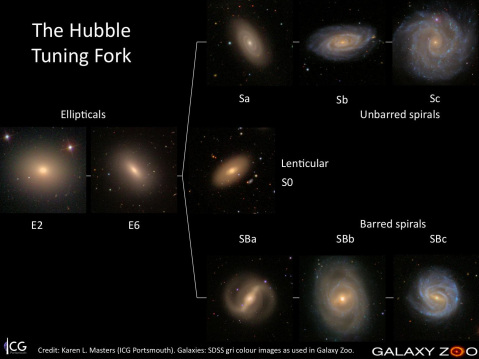
\includegraphics[width=5in]{Figures/Masters_tuningfork.jpg}
\caption[Hubble tuning fork]{The Hubble ``tuning fork'' with example images for each galaxy type created from $gri$-composite SDSS imaging. Credit: Karen L. Masters and the Sloan Digital Sky Survey (SDSS) Collaboration.}
\label{fig: tuning fork}
\end{figure}

The oldest and arguably simplest system for categorizing galaxy morphology dates back to the 1930s and Edwin Hubble's famous ``tuning fork'' \citep{Hubble1926, Hubble1936}. Based on a small sample, Hubble classified galaxies into two major groups, elliptical and spiral. Visually, elliptical galaxies possess a smooth light distribution, while spirals are characterized by a well-defined disk structure often with spiral arms. Hubble assigned a number to elliptical galaxies denoting the degree of their ellipticity, where 0 corresponds to a nearly perfectly round galaxy and 7 being highly elongated. Spirals were given additional designation in the form of letters `a' through `c', characterizing the compactness of their spiral arms. For example, ``Sa'' galaxies are tightly wound, whereas ``Sc'' spirals are looser. The spiral category was then further subdivided by galaxies that exhibited a central bar. There are also indications that the bulges inherent to many spiral galaxies share a close connection to elliptical galaxies, thus the transitional ``S0'' category: galaxies with disks that are dominated by the bulge component. 

It became common to call galaxies on the left side of the diagram ``early-types,'' and those on the right ``late-types''. Contrary to this author's belief, Hubble never intended these designations to imply galactic evolution. Instead, this terminology was borrowed from stars, where massive O and B stars were referred to as ``early-type,'' while older stars were known as ``late-type''\citep{Buta2011}. It has subsequently become clear that, much to the contrary, ellipticals are dominated by late-type stars, while disk galaxies are typically composed of young, early-type stars.  Unfortunately, the misnomer has stuck. 


This method of galaxy classification was based on a small sample of which only a few percent did not conform to the basic designations originally posited by Hubble. These leftover galaxies were dubbed ``irregulars'' or ``peculiars''. It wasn't until much later that it was discovered this galaxy type was far more prevalent than Hubble originally thought, especially in the more distant universe. Since this early attempt at classification, several other systems have been put forward but most share the same basic categories \citep[e.g.,][]{deVaucouleurs1959, Conselice2006}. Indeed, even this simplistic approach has yielded nearly a hundred years of science that has advanced our understanding of galaxy formation, structure, and evolution. 
 

%%%-------------------------------------------------------
%%% SECTION: MORPHOLOGY AS A TRACER OF GALAXY EVOLUTION
%%%-------------------------------------------------------
\section{Morphology as a tracer of galaxy evolution}
\label{chap1: morph gal evolution}

That galaxies exhibit different features is obvious, but what, if anything, do those features tell us? Because we cannot observe the entire lifespan of a single galaxy, it is fair to question whether or not morphology is primarily an indicator of age, with galaxies marching starkly through the Hubble sequence, or whether dynamical processes shape that morphology. Or both. In this section we discuss some of the major roles that galaxy morphology has played in understanding the evolution and formation of these systems. 


 %Galaxy morphology is strongly correlated with galactic star formation history. Galaxies where star formation ceased gigayears ago tend to look very different from those where star formation continues at the present time. 

%%%-------------------------------------------------------
%%% SECTION:       STELLAR POPULATIONS 
%%%-------------------------------------------------------
\subsection{Stellar populations and color bi-modality}
\label{chap1: stellar populations}

At its heart, morphology simply traces an integrated 2D projection of a galaxy's light distribution. As such, it encodes information on the distribution of a galaxy's stellar, gas, and dust content. However, these components are best traced through different wavelengths of light. In the optical, it is well known that the color-luminosity distribution of galaxies is strongly bi-modal \citep{Baldry2004b}. Most galaxies fall into either the ``red sequence'' or the ``blue cloud.'' There is a distinct gap between these two galaxy populations but recent studies have shown that, though sparse, this ``green valley'' could be a region of active galactic evolution related to a possible morphological transition \citep{Schawinski2007}.

This bimodality has resulted in the now ubiquitous color-magnitude relation (CMR) \citep{Baldry2004a, Bell2004}. These distinct populations are now believed to be due to differences in stellar populations as determined by spectroscopic age indicators as well as UV and IR photometry, with the red sequence being largely composed of \textit{passive} or \textit{quiescent} galaxies characterized by old, red stellar populations and little to no star formation, while the blue cloud is full of actively star forming galaxies with young, blue stellar populations \citep{Brinchmann2004,Kauffman2003,Salim2007,Schiminovich2007}. A galaxy's morphology is tightly correlated with its color, with elliptical galaxies typically residing in the red sequence and disk galaxies inhabiting the blue cloud \citep[e.g.,][]{Strateva2001,Baldry2004b, Cirasuolo2007, Lee2013, Taylor2015}.  This dichotomy is so ubiquitous that color has been used as a proxy for morphology when acquiring the latter was impractical \citep[e.g.,][]{Shen2003, Blanton2003c}.  The top panel of Figure \ref{fig: CMR} shows an example of the color-magnitude relation for a sample of SDSS galaxies, while the bottom panel depicts a schematic of the associated morphologies \citep[adapted from][]{Kormendy2012}. 


%This so-called \textit{passive} evolution indicates that as a galaxy ages it becomes redder. A galaxy's morphology is tightly correlated with its color: massive elliptical galaxies are typically referred to as ``red and dead,'' possessing old stellar populations, while disk galaxies are generally still undergoing star formation and thus possess young, bluer stellar populations 

%Furthermore, this color bimodality correlates with luminosity resulting in the color-magnitude relation (CMR) \citep{Baldry2004a, Bell2004}. Now ubiquitous, this relation visualizes the separation of galaxy colors as a function of luminosity resulting in three main categories: the blue cloud, the red sequence and, more recently recognized, the green valley. Studies have shown that the red sequence is dominated by early-type galaxies like elliptical/S0, while disk galaxies reside in the blue cloud. 


%%%-------------------------------------------------------
%%% FIGURE:   COLOR MAGNITUDE RELATION
%%%-------------------------------------------------------
\begin{figure}
\centering
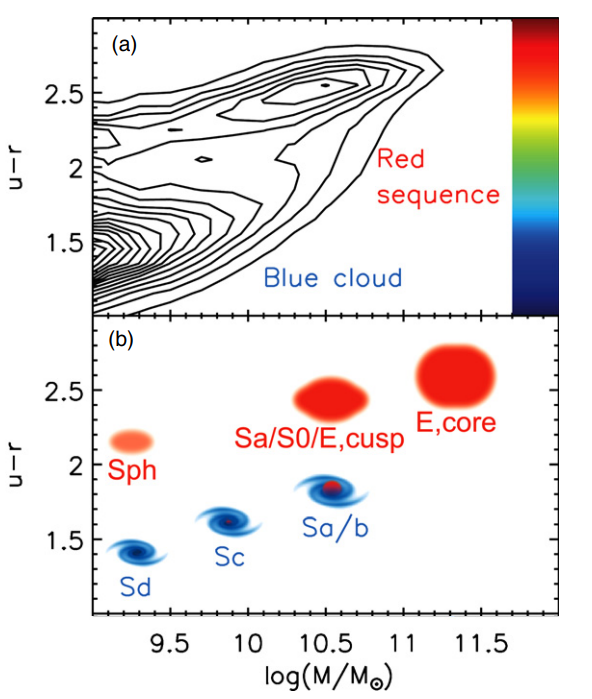
\includegraphics[width=3.5in]{Figures/kormendy_CMR.png}
\caption[Galaxy color-magnitude relation.]{Color-magnitude relation adapted from \cite{Kormendy2012}. Though the x-axis is in units of log stellar mass, mass correlates strongly with a galaxy's luminosity. The top panel shows the contours of galaxy number density \citep{Baldry2004b} with the rainbow bar denoting the associated $u-r$ color. The bottom panel depicts the dominant galaxy morphologies associated with each location.}
\label{fig: CMR}
\end{figure}


The CMR is tighter for early-type galaxies in the red sequence suggesting that this population could be coeval, having had their last epoch of star-formation at some point in the past and evolving passively thereafter \citep{Bower1992}. Studying the CMR can provide insights into the last epoch of star formation for this galaxy population \citep{Sandage1978, Tully1982}. There exists a degeneracy between the age and metallicity of stellar populations: older stars tend to be redder but this effect can also be achieved through an increase in stellar metallicity. The color dependence of the red sequence is consistent with evolution models whereby the slope is due primarily to metallicity effects \citep{Bower1992, Kodama1997}. This allows for an age estimate to be placed on the last episode of significant star formation in early-type galaxies of typically between 3-7 Gyr ago \citep[e.g.,][]{LopezCruz2004}.%The small scatter in this relation reflects that these galaxies have old, passively evolving stellar populations. 



%%%-------------------------------------------------------
%%% SECTION:  MASS ASSEMBLY
%%%-------------------------------------------------------
\subsection{Mass assembly and the emergence of the Hubble sequence}
\label{chap1: mass assembly}

Perhaps two of the most fundamental characteristics of a galaxy are its mass and its star formation rate (SFR). Though more challenging than luminosity to measure accurately, it is now thought that several processes such as feedback \citep[e.g.,][]{Gabor2010} and gas accretion \citep[e.g.,][]{Conselice2013} are directly tied to galaxy stellar mass. Thus, stellar mass functions (SMFs) are a key observable that can statistically trace the formation of stars in the universe.  A cottage industry for decades, constructing mass and lumainosity functions have provided insights into the build-up of baryonic mass over cosmic time \citep{Steidel1999,Ouchi2004,Giavalisco2004,Drory2005,Fontana2006,Marchesini2009,Caputi2011,Gonzalez2011,Lee2012,Ilbert2013,Bernardi2013,Duncan2014}. 


It is well known that the cosmic star formation rate density of the universe increased from the earliest epochs up until $z\sim2$ and has substantially declined since then, as shown in the Lilly-Madau plot in Figure \ref{fig: SFR density} \citep[and references therein]{Madau2014}. Furthermore, \cite{Madau2014} estimate that half of the stellar mass observed today was formed more than 8 Gyr ago. Understanding how this star formation was distributed among galaxy morphological types not only provides insight on the emergence of the Hubble sequence we see today, but also probes galaxy evolution and formation mechanisms as we discuss below.

\begin{figure}
\centering
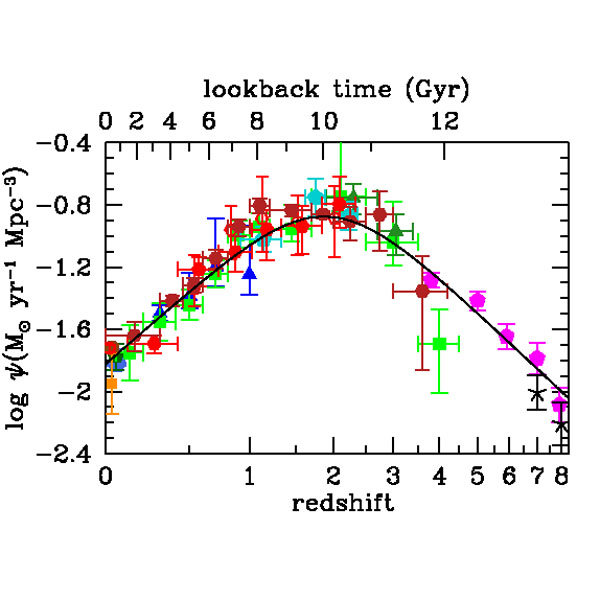
\includegraphics[width=5in]{Figures/MadauDickinson2014.jpg}
\caption[The history of cosmic star formation.]{The history of cosmic star formation as determined by FUV+IR rest-frame measurements from several galaxy samples \citep[credit:][and references therein]{Madau2014}. This shows that cosmic star formation peaked around $z\sim2$ when the universe was approximately 3.5 Gyr old followed by a gradual decline until present day.}
\label{fig: SFR density}
\end{figure}

Recent studies have shown that star-forming and quiescent galaxy types can be identified clearly up to $z\sim2$ \citep{Brammer2011, Muzzin2013}. Morphologically speaking, most of the stellar mass at $z>2$ seems to reside in irregular galaxies with the existence of disk galaxies being questionable \citep{Dickinson2000,Papovich2005,Cameron2011,Conselice2005,Conselice2011,Buitrago2013}.  Between $1<z<2$ the stellar mass density resides more in traditional disk systems but has stayed roughly constant since then \citep{Bell2004,Brammer2011,Faber2007,Muzzin2013}. Instead, SMFs indicate that the comoving number and mass density of quiescent systems has steadily increased over cosmic time with early-type systems residing as some of the most massive galaxies in the local universe \citep{Brinchmann2000, Bell2003, Bundy2005, Mortlock2013, Kelvin2014, HuertasCompany2016, Thanjavur2016}. This is peculiar as it is the star-forming population that is expected to gain in stellar mass through the birth of new stars. This finding implies that more star-forming galaxies must have their star formation quenched. 

%Recent deep surveys have shown that these two populations (star forming and quiescent) can be clearly identified at least up to z ∼ 2, and perhaps up to higher redshifts z ∼ 3–4 (Brammer et al. 2011, Muzzin et al. 2013). Intriguingly, it appears that the comoving number and mass density of quiescent galaxies has been increasing over time since z ∼ 2, while the number and mass density of star forming galaxies has stayed roughly constant or decreased during this same interval (Bell et al. 2004, 2007, Brammer et al. 2011, Faber et al. 2007, Muzzin et al. 2013). Given that it is the star forming population that is expected to be growing more massive due to the birth of new stars, this result has profound and unexpected implications — it implies that more and more star-forming galaxies must be having their star formation extinguished or “quenched” as cosmic time progresses.


Hierarchical galaxy formation predicts the build up of smaller systems before the creation of larger galaxies by way of violent mergers, simultaneously transforming disk morphologies into spheroidal systems \citep{Driver2013,Bluck2009,Man2012}. Indeed, this is likely the case in the high-redshift universe, but after $z<2$, the dominant mechanism for galaxy evolution switches to gas accretion from the intergalactic medium and with it, the formation of disk galaxies from irregular systems \citep{Conselice2013}. Both mergers and gas accretion processes are observed to be mass-dependent with the most massive galaxies settling into the familiar Hubble sequence more quickly than low-mass galaxies \citep{Buitrago2013,Conselice2011,Mortlock2013}. This so-called ``downsizing'' process, though seemingly contradictory to the hierarchical theory, is nevertheless favored observationally \citep{Cowie1996, Brinchmann2000, Bundy2005, Cimatti2006}. 



%%%-------------------------------------------------------
%%% SECTION:   MORPHOLOGY AND ENVIRONMENT
%%%-------------------------------------------------------
\subsection{Morphology as a function of environment}
\label{chap1: environment}

Several studies have demonstrated that the probability for a galaxy to be quiescent depends on its stellar mass and large-scale environment \citep{Balogh2004, Hogg2004, Peng2010, Woo2013}. That a galaxy's environment has a direct relationship with its morphology was first quantified by \cite{Dressler1980}, and is known as the morphology-density relation. This empirical relation finds that elliptical galaxies tend to reside in the densest environments, i.e., rich groups and clusters, at all stages of cosmic time, while disks reside in isolated environments. This strongly indicates that environment plays a crucial role in galaxy evolution \citep[e.g.,][]{Fasano2000, Smith2005, Peng2010}. 

Of particular interest, \cite{Peng2010} demonstrate that the fraction of quiescent galaxies in dense regions relies on different physical mechanisms depending on whether galaxies were central to the group or merely a satellite. Specifically, they find that the fraction of quiescent centrals is dependent solely on stellar mass, while that for satellites is dependent on both stellar mass and environment. There are several processes that could preferentially suppress star formation in satellite galaxies including harassment \citep{Moore1996}, tidal stripping or ``strangulation'' \citep{Kawata2008}, and ram pressure stripping \citep{Gunn1972}. Another curious observational result is that of ``galactic conformity,'' in which halos with red central galaxies preferentially have red satellites \citep{Weinmann2006}. There is currently little consensus on the physics that drive this phenomena \citep{Kauffmann2013,Hearin2015,Hearin2016,Pahwa2017} but it is clear that the relationship between morphology and environment continues to advance our understanding of galaxy evolution.

%Much study has been done to separate the effects of environment from mass, i.e., secular, causes of morphological features. Peng, Shen,,etc. Cluster environments are, compared to the field, extremely hot and dense. Galaxies residing in these environments have faster velocity , on average.   It's estimated that field galaxies are, on average, 1 per Mpc (?). The merging rate depends on the density of galaxies. In the past galaxies were closer together so merging was a bigger deal. Logically then, it would seem that merging happens all the time in clusters and that this subsequently causes a morphological change from disk to elliptical. However, galaxies are moving so briskly in clusters that it becomes less likely that they collide! Instead, mergers seems to be a predominant morphological mechanism in groups rather than clusters. In clusters, instead, other physical processes shape the way a galaxy evolves and looks over time. 

%environmental processes including satellite quenching (Lagos et al. 2014,Rafieferantsoa et al. 2014)

%Certainly there are many candidate processes that could preferentially quenchsatellites, such as harrassment, tidal stripping, or ram pressure stripping. In many SAMs, galaxies are not allowed to accrete any new gas from the hot halo or the IGM once they become satellites (sometimes called “strangulation”). This is known to produce far too high a fraction of quiescent satellites (Font et al. 2008, Kimm et al. 2009, Weinmann et al.2006b). Instead, satellite quenching seems to take a surprisingly long time, perhaps many Gyr (Wetzel et al. 2012). Hydrodynamic simulations indeed show that infalling satellites remain star-forming for at least a Gyr (Simha et al. 2009), as it takes time for the hot gas and dark matter from the halo in which the satellite galaxy was born to be stripped away. Including this delayed stripping of the hot gas halo, without including any other environmental effects (e.g. tidal or ram pressure stripping of the cold gas in satellites) improves satellite statistics iit SAMs (Font et al. 2008, Weinmann et al. 2010), though some tension with observations remains (Hirschmann et al. 2014). A particularly curious observational result is “galaxy conformity”, in which halos with red central galaxies preferentially have red satellites (Weinmann et al. 2006a). 



%%%-------------------------------------------------------
%%% SECTION:    RARE MORPHOLOGIES
%%%-------------------------------------------------------
\subsection{Insights from rare morphologies}

While great insight into the formation and evolution of galaxies has been gleaned through examination of broad morphological categories, more can be learned by digging into the details. Any theory of galaxy evolution will have to account for the dizzying array of galactic forms including the development of bars, bulges, and rings, as well as rare morphologies such as the ``green peas,'' or giant clumps of star formation in galaxies in the nearby universe discussed below.

Identifying finer galactic structures has become easier with the advent of cameras such as the Wide Field Camera 3 \citep{Dressel2012} aboard the Hubble Space Telescope, which has imaged the universe in unprecedented detail. However, it has only been since the development of large scale surveys like, for example, the Sloan Digital Sky Survey \citep[SDSS,][]{York2000,Abazajian2003}, the Cosmic Assembly and Near-infrared Deep Extragalactic Legacy Survey \citep[CANDELS,][]{Grogin2011,Koekemoer2011}, and the Dark Energy Survey \citep[DES,][]{DES2005} that astronomers have become aware of rare populations of galaxies. While small, these populations provide a means to constrain formation and evolution theories. 

First recognized as an individual class of galaxies by Galaxy Zoo volunteers in 2007, the ``green peas'' are a type of luminous blue compact galaxy whose name reflects the hue of these galaxies in the false color SDSS images presented during the Galaxy Zoo project \citep{Lintott2008,Cardamone2009}. These oxygen-rich objects are observed to have some of the largest star formation rates with some of the smallest masses \citep{Amorin2010}. It is surmised that these galaxies were commonplace in the early universe and likely played a large role in the reionization of the universe \citep{Izotov2016}. That such galaxies exist in the local universe provides a way to probe the cosmic past. 

Another class of potential local analogs of high-redshift counterparts are low redshift ``clumpy'' galaxies \citep{Elmegreen2005,Elmegreen2013}. As previously discussed, galaxies of the past were largely irregular with star formation rates much higher than today \citep{Madau2014}. Much of the peculiar shapes of these galaxies are due to massive knots of star formation \citep{Guo2015}. These galaxies underwent processes that transformed them into disk galaxies with the result being that this particular morphology is rather rare in the local universe. These star-forming clumps are thought to form via gravitational disk instability \citep{Toomre1964}. If these features are long-lived compared to their host galaxy, it is possible they contribute to the growth of the galactic bulge \citep{Conselice2014}. Chapter \ref{chap:5} presents a more in depth discussion and preliminary analysis of a sample of such galaxies discovered through the Galaxy Zoo project.


\section{Obtaining morphologies}
\label{chap1: obtaining morphologies}

A galaxy's morphology is an integral component for understanding the nature of these systems as well as deriving a fuller comprehension of their formation and evolution. However, obtaining such morphological information poses several challenges. This section will discuss the methods in which galaxy morphologies are collected and quantified. 

\subsection{Visual classifications}
\label{chap1: visual}

For most of the past century, galaxy morphologies were determined by a small number of expert astronomers beginning with Hubble. Visual classification, though highly accurate due to the human mind's unique pattern recognition capability is, however, incredibly time consuming. For decades, assignment of morphological type to galaxies resulted in small samples with varying degrees of descriptive complexity and often lacking in statistical significance \citep{Hubble1936, Sandage1961, SandageTammann1981, deVaucouleurs1963, deVaucouleurs1991}. With surveys like the Sloan Digital Sky Survey \citep[SDSS,][]{Abazajian2003} and the Canada-France-Hawaii Telescope Legacy Survey \citep{Gwyn2012}, coupled with cartels of graduate student classifiers, samples approached the tens of thousands \citep{Fukugita2007, Schawinski2007, NairAbraham2010}.

Unfortunately, this approach still cannot take full advantage of the depth and scope of such large scale surveys. This necessitated the birth of the Galaxy Zoo (GZ) project \citep{Lintott2008, Lintott2011, Willett2013, Willett2017, Simmons2017}, the first effort to crowd-source the task of galaxy morphology to the general public. With the efforts of hundreds of thousands of citizen scientists, GZ has released visual morphologies for over one million galaxies, providing a solution that scales visual classification for current surveys and producing a prolific amount of scientific output \citep[e.g.,][]{Land2008, Bamford2009, Darg2010, Schawinski2014, Galloway2015, Smethurst2016}.
A hybrid approach is the system developed by the CANDELS \citep{Grogin2011, Koekemoer2011} team for imaging produced by the Hubble Space Telescope. This scheme \citep{Kartaltepe2015} crowd-sources not to the general public, but to dozens of expert astronomers, collecting visual classifications for over 50,000 galaxies in the CANDELS fields. 
%upcoming surveys such as \textit{LSST} and \textit{Euclid} will require a different approach, imaging more than a billion new galaxies  \citep{LSST, Euclid}.  If detailed morphologies can be extracted for just  0.1\% of this imaging, we will have millions of images to contend with. A project of this magnitude would take more than sixty years to classify at Galaxy Zoo's current rate and configuration. Standard visual morphology methods will thus be unable to cope with the scale of data. 


\subsection{Automated classifications}
\label{chap1: automated}

Another approach has been the automated extraction of morphologies with the development of parametric \citep{Sersic1968, Odewahn2002, Peng2002}, and non-parametric 
\citep{Abraham1994, 
	   Conselice2003, 
	   Abraham2003, 
	   Lotz2004,  
	   Freeman2013} 
structural indicators. While these scale well to large samples 
\citep[e.g.,][]{Simard2011, 
			Griffith2012, 
			Casteels2014, 
			Holwerda2014, 
			Meert2016}, 
they often fail to capture detailed structure and can provide only statistical morphologies with large uncertainties \cite[e.g.,][]{Abraham1996, Bershady2000}. We briefly highlight a few of these indicators here while a more detailed discussion can be found in Chapter \ref{chap:2}. 

One of the first and most popular parametric approaches for modeling a galaxy's light distribution is the S\'ersic profile:
\begin{equation}
I(R) = I_e \exp \Big\{-b_n\Big[\Big(\frac{R}{R_e}\Big)^{1/n}-1\Big]\Big\}
\end{equation}
where $I_e$ is the intensity at the ``effective'' radius $R_e$ that encloses half of the total light from the model, $n$ is the S\'ersic index that essentially describes the concentration of the light profile, and $b_n$ is a term that depends on $n$. The de Vaucouleurs law is produced when $n=4$, which well describes the light profile of elliptical galaxies \citep{deVaucouleurs1948}. On the other hand, a Sersic index of $n=1$ reduces the equation to an exponential which is a good description for disk galaxies. This index has been used for decades as a broad method to classify galaxies into early- and late-type categories. 

A drawback to the parametric approach is the need to assume the underlying distribution and while this technique works well for galaxies that are obviously elliptical or spiral, it produces mixed results for other morphological types, i.e., irregulars or peculiars, which have low central concentration resulting in a low Sersic index, but which do not have disks or spiral arms. Additionally, fitting this function to thousands or even millions of galaxies is time consuming. Non-parametric structural indicators require fewer assumptions and are derived empirically.

Closely related to the S\'ersic index is the non-parametric diagnostic of concentration. Originally conceived by \cite{Abraham1996}, it has several definitions but each measures the ratio of the aggregated light within two concentric apertures about the galaxy's center: one close to the galaxy's center and another further out. Typically, these apertures contain 50\% and 90\% of the galaxy's total light. Measuring a galaxy's concentration can be much faster than fitting it with a S\'ersic profile and less prone to fitting failures. 

Once these parametric and non-parametric diagnostics have been computed for a sample of galaxies it is then common practice to place a cut on one or more of these parameters to separate the sample into early- and late-types \citep{Shen2003}. More sophisticated approaches involve measuring several automated diagnostics and separating galaxies in a two dimensional plane, a technique that has been highly successful at identifying not only distinctions between spheroidal and disk-like galaxies but also merging and interacting systems \citep{Lotz2004, Conselice2000, Conselice2003,Freeman2013}. 


 %Several of these diagnostics have been developed over the past couple decades, each probing a different part of the galaxy's light profile and thus its overall dynamical distribution. The most common diagnostics are described in greater detail in Chapter 2. 
%Example of using parametric Sersic profile to classify galaxies as early-/late-type: ``We show that the wavelength-dependence of n may be employed to separate visually-classified early- and late-type galaxies in a manner similar to the use of colour and n. Furthermore, we find that the wavelength variation of n can recover galaxies that are misclassified by these other morphological proxies."\citep{Vika2015}


\subsection{Machine learning}
\label{chap1: machine learning}

Machine learning techniques are becoming increasingly popular for classification and image processing tasks. Another automated approach, these generally work by defining a set of features that describe the morphology in an $N$-dimensional space. These features can be anything: color, mass, spectral index, velocity dispersion, and of course the parametric and non-parametric indicators discussed above. Choosing which features are most appropriate will depend on the classification task at hand, the particular machine learning algorithm chosen, and the strength of the correlation between a given feature and the galaxy's intended class. 

The location in this $N$-dimensional morphology space defines a morphological type for each galaxy. Learning the morphology space can be achieved through algorithms such as Support Vector Machines \citep{HuertasCompany2008} or Principal Component Analysis \citep{Watanabe1985, Conselice2006, Scarlata2007, Peth2016}. Another approach is through deep learning, a machine learning technique that attempts to model high level abstractions. Algorithms like convolutional and artificial neural networks (CNNs, ANNs) have been used for galaxy morphology classification with impressive accuracy \citep{Ball2004, 	Banerji2010, Dieleman2015, HuertasCompany2015,DominguezSanchez2017}. 

A drawback to all machine learning classification techniques is the need for standardized training data, with more complex algorithms requiring more data. Furthermore, these data are best when consistent for each survey: differences in resolution and depth can be implicitly learned by the algorithm making their application to disparate surveys challenging. 


\section{Overview of Galaxy Zoo: Express}
\label{chap1: gzx}

In this thesis we present a system that preserves the best features of both visual and automatic classifications, developing for the first time a framework that brings both human and machine intelligence to the task of galaxy morphology to handle the scale and scope of next generation data. We demonstrate the effectiveness of such a system through a re-analysis of visual galaxy morphology classifications collected during the Galaxy Zoo 2 project, and combine these with a Random Forest machine learning algorithm that trains on a suite of non-parametric morphology indicators widely used for automated morphologies.  We demonstrate that our method provides a factor of 11.4 increase in the rate of galaxy morphology classification  while maintaining at least 93.1\% classification accuracy as compared to Galaxy Zoo 2 published data. Here we present an overview of our framework, which also serves as a blueprint for this thesis. 
%In this work we focus on the first question of the Galaxy Zoo decision tree.

%%%-------------------------------------------------------
%%% FIGURE:     GZ EXPRESS Schematic
%%%-------------------------------------------------------
\begin{figure*}
%\figurenum{1}
\plotone{Figures/human_machine/f1.pdf}
\caption[Schematic of the Galaxy Zoo: Express human+machine hybrid system.]{Schematic of our hybrid system. Humans provide classifications of galaxy images via a web interface. We simulate this with the Galaxy Zoo 2 classification data described in Chapter~\ref{chap:2}. Human classifications are processed with an algorithm described in Chapter~\ref{chap:3}. Subjects that pass a set of thresholds are considered human-retired (fully classified) and provide the training sample for the machine classifier as described in Chapter \ref{chap:4}. The trained machine is applied to all subjects not yet retired. Those that pass an analogous set of machine-specific thresholds are considered machine-retired. The rest remain in the system to be classified by either human or machine. This procedure is repeated  nightly. \label{fig: schematic}}
\end{figure*}


%%----------------------------------------------------------------------------------------------------------------------------------------------------
%%   GALAXY ZOO EXPRESS OVERVIEW
%%---------------------------------------------------------------------------------------------------------------------------------------------------

The Galaxy Zoo Express (GZX) framework combines human and machine to increase morphological classification efficiency, both in terms of the classification rate and required human effort. Figure~\ref{fig: schematic} presents a schematic of GZX including section numbers as a shortcut for the reader. We note that transparent portions  of the schematic represent areas of future work which we explore in Chapter \ref{chap:summary}. Any system combining human and machine classifications will have a set of generic features: a group of human classifiers, at least one machine classifier, and a decision engine which determines how these classifications should be combined.

In this work we demonstrate our system through a re-analysis of  Galaxy Zoo 2 (GZ2) classifications. This allows us to  create simulations of human classifiers. These classifications are used most effectively when processed with SWAP, a Bayesian code described in Chapter \ref{chap:3}, first developed for the Space Warps gravitational lens discovery project~\citep{Marshall2016}. These subjects provide the machine's training sample. 

In Chapter~\ref{chap:4}, we incorporate a machine classifier. We have developed a Random Forest algorithm that trains on measured morphology indicators (discussed in Chapter \ref{chap:2}) such as concentration, asymmetry, Gini coefficient, and \M{20}, well-suited for the top-level question of the GZ2 decision tree. After a sufficient number of subjects have been classified by humans, the machine is trained and its performance assessed through cross-validation. This procedure is repeated nightly and the machine's performance increases with the size of the training sample, albeit with a performance limit. Once the machine reaches an acceptable level of performance it is applied to the remaining galaxy sample. 

Even with this simple description, one can see that the classification process will progress in three phases.  First, the machine will not yet have reached an acceptable level of performance; only humans contribute to subject classification. Second, the machine's performance will improve; both humans and machine will be responsible for classification. Finally, machine performance will slow; remaining images will likely need to be classified by humans. This blueprint allows even modest machine learning routines to make significant contributions alongside human classifiers and removes the need for ever-increasing performance in machine classification.